\documentclass[10pt,a4paper,onecolumn]{article}
\usepackage{marginnote}
\usepackage{graphicx}
\usepackage{xcolor}
\usepackage{authblk,etoolbox}
\usepackage{titlesec}
\usepackage{calc}
\usepackage{tikz}
\usepackage{hyperref}
\hypersetup{colorlinks,breaklinks,
            urlcolor=[rgb]{0.0, 0.5, 1.0},
            linkcolor=[rgb]{0.0, 0.5, 1.0}}
\usepackage{caption}
\usepackage{tcolorbox}
\usepackage{amssymb,amsmath}
\usepackage{ifxetex,ifluatex}
\usepackage{seqsplit}
\usepackage{xstring}

\usepackage{float}
\let\origfigure\figure
\let\endorigfigure\endfigure
\renewenvironment{figure}[1][2] {
    \expandafter\origfigure\expandafter[H]
} {
    \endorigfigure
}

\usepackage{fixltx2e} % provides \textsubscript
\usepackage[
  backend=biber,
%  style=alphabetic,
%  citestyle=numeric
]{biblatex}
\bibliography{paper.bib}

% --- Splitting \texttt --------------------------------------------------

\let\textttOrig=\texttt
\def\texttt#1{\expandafter\textttOrig{\seqsplit{#1}}}
\renewcommand{\seqinsert}{\ifmmode
  \allowbreak
  \else\penalty6000\hspace{0pt plus 0.02em}\fi}


% --- Pandoc does not distinguish between links like [foo](bar) and
% --- [foo](foo) -- a simplistic Markdown model.  However, this is
% --- wrong:  in links like [foo](foo) the text is the url, and must
% --- be split correspondingly.
% --- Here we detect links \href{foo}{foo}, and also links starting
% --- with https://doi.org, and use path-like splitting (but not
% --- escaping!) with these links.
% --- Another vile thing pandoc does is the different escaping of
% --- foo and bar.  This may confound our detection.
% --- This problem we do not try to solve at present, with the exception
% --- of doi-like urls, which we detect correctly.


\makeatletter
\let\href@Orig=\href
\def\href@Urllike#1#2{\href@Orig{#1}{\begingroup
    \def\Url@String{#2}\Url@FormatString
    \endgroup}}
\def\href@Notdoi#1#2{\def\tempa{#1}\def\tempb{#2}%
  \ifx\tempa\tempb\relax\href@Urllike{#1}{#2}\else
  \href@Orig{#1}{#2}\fi}
\def\href#1#2{%
  \IfBeginWith{#1}{https://doi.org}%
  {\href@Urllike{#1}{#2}}{\href@Notdoi{#1}{#2}}}
\makeatother

\newlength{\cslhangindent}
\setlength{\cslhangindent}{1.5em}
\newlength{\csllabelwidth}
\setlength{\csllabelwidth}{3em}
\newenvironment{CSLReferences}[3] % #1 hanging-ident, #2 entry spacing
 {% don't indent paragraphs
  \setlength{\parindent}{0pt}
  % turn on hanging indent if param 1 is 1
  \ifodd #1 \everypar{\setlength{\hangindent}{\cslhangindent}}\ignorespaces\fi
  % set entry spacing
  \ifnum #2 > 0
  \setlength{\parskip}{#2\baselineskip}
  \fi
 }%
 {}
\usepackage{calc}
\newcommand{\CSLBlock}[1]{#1\hfill\break}
\newcommand{\CSLLeftMargin}[1]{\parbox[t]{\csllabelwidth}{#1}}
\newcommand{\CSLRightInline}[1]{\parbox[t]{\linewidth - \csllabelwidth}{#1}}
\newcommand{\CSLIndent}[1]{\hspace{\cslhangindent}#1}

% --- Page layout -------------------------------------------------------------
\usepackage[top=3.5cm, bottom=3cm, right=1.5cm, left=1.0cm,
            headheight=2.2cm, reversemp, includemp, marginparwidth=4.5cm]{geometry}

% --- Default font ------------------------------------------------------------
% \renewcommand\familydefault{\sfdefault}

% --- Style -------------------------------------------------------------------
\renewcommand{\bibfont}{\small \sffamily}
\renewcommand{\captionfont}{\small\sffamily}
\renewcommand{\captionlabelfont}{\bfseries}

% --- Section/SubSection/SubSubSection ----------------------------------------
\titleformat{\section}
  {\normalfont\sffamily\Large\bfseries}
  {}{0pt}{}
\titleformat{\subsection}
  {\normalfont\sffamily\large\bfseries}
  {}{0pt}{}
\titleformat{\subsubsection}
  {\normalfont\sffamily\bfseries}
  {}{0pt}{}
\titleformat*{\paragraph}
  {\sffamily\normalsize}


% --- Header / Footer ---------------------------------------------------------
\usepackage{fancyhdr}
\pagestyle{fancy}
\fancyhf{}
%\renewcommand{\headrulewidth}{0.50pt}
\renewcommand{\headrulewidth}{0pt}
\fancyhead[L]{\hspace{-0.75cm}
\includegraphics[width=5.5cm]{joss-logo.png}}
\fancyhead[C]{}
\fancyhead[R]{}
\renewcommand{\footrulewidth}{0.25pt}

\fancyfoot[L]{\parbox[t]{0.98\headwidth}{\footnotesize{\sffamily , (2023). Atmospheric
Retrievals with
petitRADTRANS. \textit{Journal of Open Source Software}, ''(''), ''. \url{https://doi.org/10.5281/zenodo.8337871}}}}


\fancyfoot[R]{\sffamily \thepage}
\makeatletter
\let\ps@plain\ps@fancy
\fancyheadoffset[L]{4.5cm}
\fancyfootoffset[L]{4.5cm}

% --- Macros ---------

\definecolor{linky}{rgb}{0.0, 0.5, 1.0}

\newtcolorbox{repobox}
   {colback=red, colframe=red!75!black,
     boxrule=0.5pt, arc=2pt, left=6pt, right=6pt, top=3pt, bottom=3pt}

\newcommand{\ExternalLink}{%
   \tikz[x=1.2ex, y=1.2ex, baseline=-0.05ex]{%
       \begin{scope}[x=1ex, y=1ex]
           \clip (-0.1,-0.1)
               --++ (-0, 1.2)
               --++ (0.6, 0)
               --++ (0, -0.6)
               --++ (0.6, 0)
               --++ (0, -1);
           \path[draw,
               line width = 0.5,
               rounded corners=0.5]
               (0,0) rectangle (1,1);
       \end{scope}
       \path[draw, line width = 0.5] (0.5, 0.5)
           -- (1, 1);
       \path[draw, line width = 0.5] (0.6, 1)
           -- (1, 1) -- (1, 0.6);
       }
   }

% --- Title / Authors ---------------------------------------------------------
% patch \maketitle so that it doesn't center
\patchcmd{\@maketitle}{center}{flushleft}{}{}
\patchcmd{\@maketitle}{center}{flushleft}{}{}
% patch \maketitle so that the font size for the title is normal
\patchcmd{\@maketitle}{\LARGE}{\LARGE\sffamily}{}{}
% patch the patch by authblk so that the author block is flush left
\def\maketitle{{%
  \renewenvironment{tabular}[2][]
    {\begin{flushleft}}
    {\end{flushleft}}
  \AB@maketitle}}
\makeatletter
\renewcommand\AB@affilsepx{ \protect\Affilfont}
%\renewcommand\AB@affilnote[1]{{\bfseries #1}\hspace{2pt}}
\renewcommand\AB@affilnote[1]{{\bfseries #1}\hspace{3pt}}
\renewcommand{\affil}[2][]%
   {\newaffiltrue\let\AB@blk@and\AB@pand
      \if\relax#1\relax\def\AB@note{\AB@thenote}\else\def\AB@note{#1}%
        \setcounter{Maxaffil}{0}\fi
        \begingroup
        \let\href=\href@Orig
        \let\texttt=\textttOrig
        \let\protect\@unexpandable@protect
        \def\thanks{\protect\thanks}\def\footnote{\protect\footnote}%
        \@temptokena=\expandafter{\AB@authors}%
        {\def\\{\protect\\\protect\Affilfont}\xdef\AB@temp{#2}}%
         \xdef\AB@authors{\the\@temptokena\AB@las\AB@au@str
         \protect\\[\affilsep]\protect\Affilfont\AB@temp}%
         \gdef\AB@las{}\gdef\AB@au@str{}%
        {\def\\{, \ignorespaces}\xdef\AB@temp{#2}}%
        \@temptokena=\expandafter{\AB@affillist}%
        \xdef\AB@affillist{\the\@temptokena \AB@affilsep
          \AB@affilnote{\AB@note}\protect\Affilfont\AB@temp}%
      \endgroup
       \let\AB@affilsep\AB@affilsepx
}
\makeatother
\renewcommand\Authfont{\sffamily\bfseries}
\renewcommand\Affilfont{\sffamily\small\mdseries}
\setlength{\affilsep}{1em}


\ifnum 0\ifxetex 1\fi\ifluatex 1\fi=0 % if pdftex
  \usepackage[T1]{fontenc}
  \usepackage[utf8]{inputenc}

\else % if luatex or xelatex
  \ifxetex
    \usepackage{mathspec}
  \else
    \usepackage{fontspec}
  \fi
  \defaultfontfeatures{Ligatures=TeX,Scale=MatchLowercase}

\fi
% use upquote if available, for straight quotes in verbatim environments
\IfFileExists{upquote.sty}{\usepackage{upquote}}{}
% use microtype if available
\IfFileExists{microtype.sty}{%
\usepackage{microtype}
\UseMicrotypeSet[protrusion]{basicmath} % disable protrusion for tt fonts
}{}

\usepackage{hyperref}
\hypersetup{unicode=true,
            pdftitle={Atmospheric Retrievals with petitRADTRANS},
            pdfborder={0 0 0},
            breaklinks=true}
\urlstyle{same}  % don't use monospace font for urls

% --- We redefined \texttt, but in sections and captions we want the
% --- old definition
\let\addcontentslineOrig=\addcontentsline
\def\addcontentsline#1#2#3{\bgroup
  \let\texttt=\textttOrig\addcontentslineOrig{#1}{#2}{#3}\egroup}
\let\markbothOrig\markboth
\def\markboth#1#2{\bgroup
  \let\texttt=\textttOrig\markbothOrig{#1}{#2}\egroup}
\let\markrightOrig\markright
\def\markright#1{\bgroup
  \let\texttt=\textttOrig\markrightOrig{#1}\egroup}


\usepackage{graphicx,grffile}
\makeatletter
\def\maxwidth{\ifdim\Gin@nat@width>\linewidth\linewidth\else\Gin@nat@width\fi}
\def\maxheight{\ifdim\Gin@nat@height>\textheight\textheight\else\Gin@nat@height\fi}
\makeatother
% Scale images if necessary, so that they will not overflow the page
% margins by default, and it is still possible to overwrite the defaults
% using explicit options in \includegraphics[width, height, ...]{}
\setkeys{Gin}{width=\maxwidth,height=\maxheight,keepaspectratio}
\IfFileExists{parskip.sty}{%
\usepackage{parskip}
}{% else
\setlength{\parindent}{0pt}
\setlength{\parskip}{6pt plus 2pt minus 1pt}
}
\setlength{\emergencystretch}{3em}  % prevent overfull lines
\providecommand{\tightlist}{%
  \setlength{\itemsep}{0pt}\setlength{\parskip}{0pt}}
\setcounter{secnumdepth}{0}
% Redefines (sub)paragraphs to behave more like sections
\ifx\paragraph\undefined\else
\let\oldparagraph\paragraph
\renewcommand{\paragraph}[1]{\oldparagraph{#1}\mbox{}}
\fi
\ifx\subparagraph\undefined\else
\let\oldsubparagraph\subparagraph
\renewcommand{\subparagraph}[1]{\oldsubparagraph{#1}\mbox{}}
\fi

\title{Atmospheric Retrievals with petitRADTRANS}

        \author[1]{Evert Nasedkin}
          \author[1]{Paul Mollière}
          \author[1]{Doriann Blain}
    
      \affil[1]{Max Planck Institut für Astronomie, DE}
  \date{\vspace{-5ex}}

\begin{document}
\maketitle

\marginpar{
  \sffamily\small

  {\bfseries DOI:} \href{https://doi.org/10.5281/zenodo.8337871}{\color{linky}{10.5281/zenodo.8337871}}

  \vspace{2mm}

  {\bfseries Software}
  \begin{itemize}
    \setlength\itemsep{0em}
    \item \href{}{\color{linky}{Review}} \ExternalLink
    \item \href{https://gitlab.com/mauricemolli/petitRADTRANS}{\color{linky}{Repository}} \ExternalLink
    \item \href{http://dx.doi.org/10.5281/zenodo.8337871}{\color{linky}{Archive}} \ExternalLink
  \end{itemize}

  \vspace{2mm}

  {\bfseries Submitted:} 12 September 2023\\
  {\bfseries Published:} Unpublished

  \vspace{2mm}
  {\bfseries License}\\
  Authors of papers retain copyright and release the work under a Creative Commons Attribution 4.0 International License (\href{https://creativecommons.org/licenses/by/4.0/}{\color{linky}{CC BY 4.0}}).
}

\section{Summary}\label{summary}

\texttt{petitRADTRANS} (pRT) is a fast radiative transfer code used for
computing emission and transmission spectra of exoplanet atmospheres
(Mollière et al. 2019), combining a FORTRAN back end with a Python based
user interface. It is widely used in the exoplanet community with 161
references in the literature to date, and has been benchmarked against
numerous similar tools, including many listed in (MacDonald and Batalha
2023). The spectra calculated with pRT can be used as a forward model
for fitting spectroscopic data using Monte Carlo techniques, commonly
referred to as an atmospheric retrieval (Madhusudhan and Seager 2009).
The new retrieval module combines fast forward modelling with nested
sampling codes, allowing for atmospheric retrievals on a large range of
different types of exoplanet data. Thus it is now possible to use pRT to
easily and quickly infer the atmospheric properties of exoplanets in
both transmission and thermal emission.

\section{Statement of need}\label{statement-of-need}

Atmospheric retrievals are a cornerstone of exoplanet atmospheric
characterisation. pRT provides a powerful and user-friendly tool for
researchers to fit exoplanet spectra with a range of built in or custom
atmospheric models. Various thermal structures, chemistry and cloud
parameterisations and opacity calculation methods can be combined and
used to perform parameter estimation and model comparison for a given
atmospheric spectrum. With increasing volumes of both ground- and
space-based spectra available, it is necessary for exoplanet researchers
to have access to a range of characterisation tools.

\section{petitRADTANS Retrieval
Module}\label{petitradtans-retrieval-module}

The \texttt{Retrieval} module combines the \texttt{Radtrans} forward
modelling class with a nested sampler via a likelihood function to
perform an atmospheric retrieval. Both \texttt{MultiNest} (F. Feroz and
Hobson 2008; F. Feroz, Hobson, and Bridges 2009; Farhan Feroz et al.
2019; J. Buchner et al. 2014) and \texttt{Ultranest} (J. Buchner et al.
2014; Johannes Buchner 2019) samplers are available, with both offering
MPI implementations that allow for easy parallelisation.

Datasets, priors and other retrieval hyper parameters are set through
the \texttt{RetrievalConfig} class, while the \texttt{models} module
includes a range of complete atmospheric models that can be fit to the
data. Users can also define their own model function, either by making
use of temperature profiles from the \texttt{physics} module and
chemistry parameterisations from the \texttt{chemistry} module or by
implementing their own forward model.

\begin{figure}
\centering
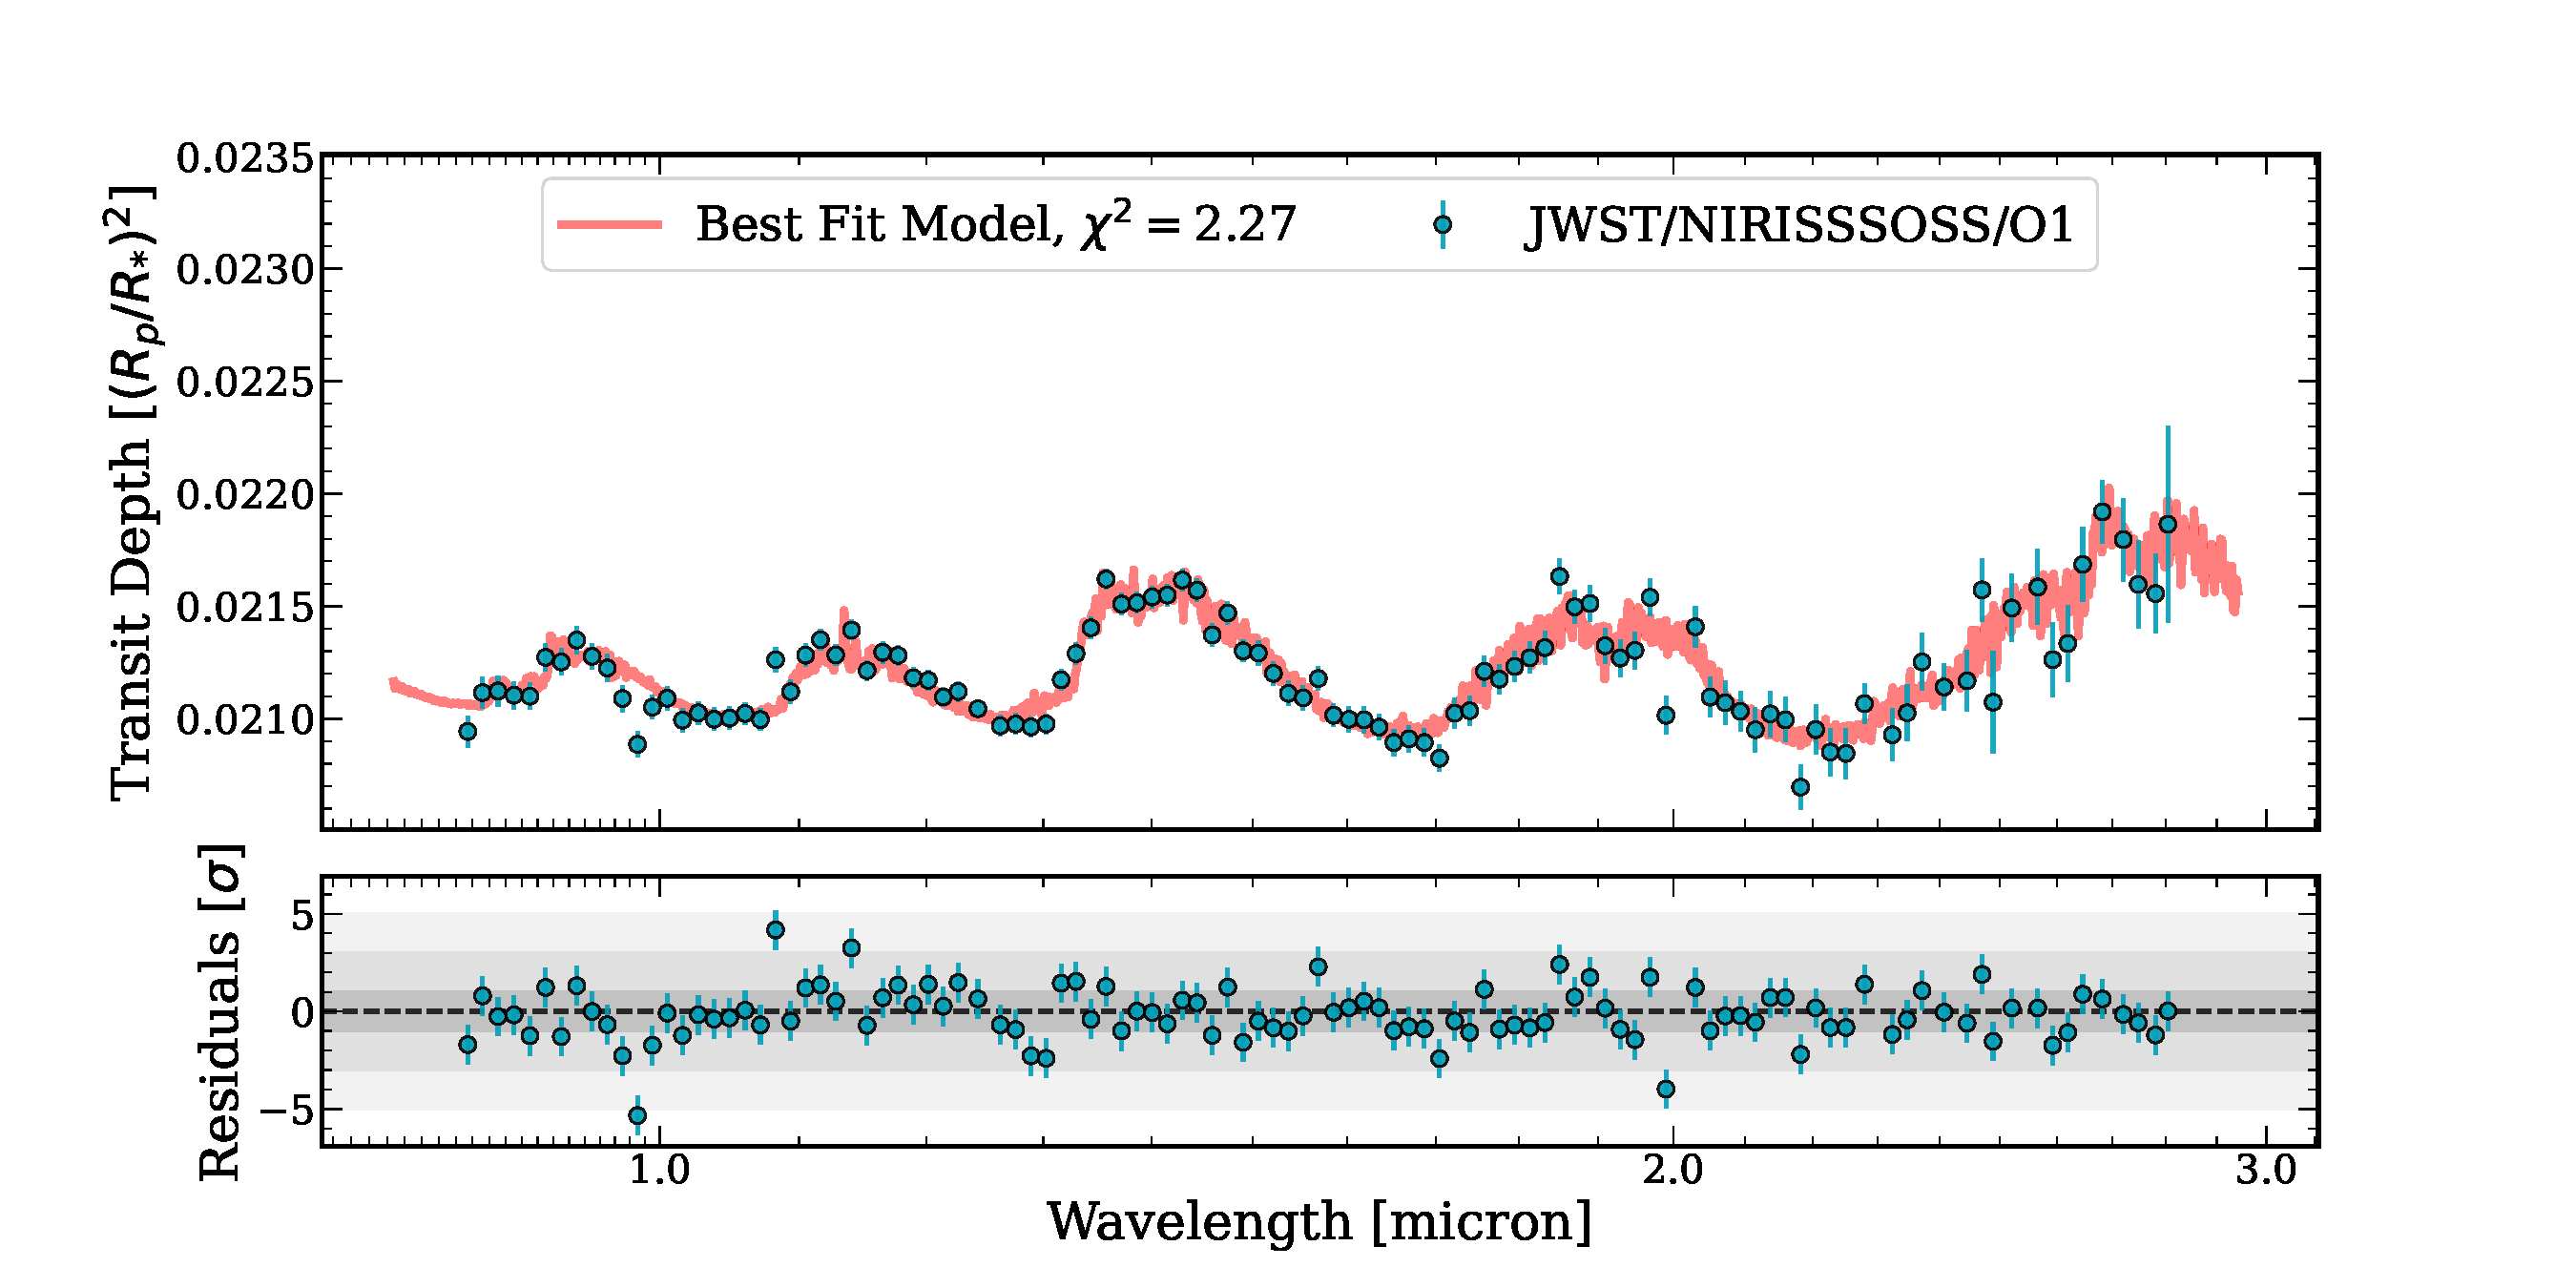
\includegraphics{WASP39b_NIRISSSOSSO1_typical_bestfit_spec.pdf}
\caption{Typical example of default pRT outputs. This highlights the fit
of a transmission spectrum model to JWST/NIRISS/SOSS data of WASP 39 b
as part of the Transiting Early Release Science
program.\label{fig:WASP39}}
\end{figure}

Multiple datasets can be included into a single retrieval, with each
dataset receiving its own \texttt{Radtrans} object used for the
radiative transfer calculation where some or all forward model
parameters may be shared between the different data sets. This allows
for highly flexible retrievals where multiple spectral resolutions,
wavelength ranges and even atmospheric models can be combined in a
single retrieval. Each dataset can also receive scaling factors (for the
flux, uncertainties or both), error inflation factors and offsets. The
model functions are used to compute a spectrum \(\vec{S}\), which is
convolved to the instrumental resolution and binned to the wavelength
bins of the data using a custom binning function to account for
non-uniform bin sizes. The resulting spectrum compared to the data with
flux \(\vec{F}\) and covariance \(\mathbf{C}\) in the likelihood
function: \begin{equation}\label{eqn:loglike}
    -2\log\mathcal{L} = \left(\vec{S}-\vec{F}\right)^{T}\mathbf{C}^{-1}\left(\vec{S}-\vec{F}\right) + \log\left(2\pi\det\left(\mathbf{C}\right)\right).
\end{equation} The second term is included in the likelihood to allow
for uncertainties to vary as a free parameter during the retrieval, and
penalizes overly large uncertainties. An likelihood function for high
resolution data based on that of (Gibson et al. 2020) is also available.

pRT can compute spectra either using line-by-line calculations, or using
correlated-k (c-k) tables for defining the opacities of molecular
species. We include up-to-date correlated-k line lists from Exomol
(Tennyson and Yurchenko 2012; McKemmish, Yurchenko, and Tennyson 2016;
Polyansky et al. 2018; Chubb et al. 2020) and HITEMP Hargreaves et al.
(2020), with the full set of available opacities listed in the online
documentation. The \verb|exo-k| package is used to resample the the
correlated-k opacity tables to a lower spectral resolution in order to
reduce the computation time (Leconte 2021). Combining the c-k opacities
of multiple species requires mixing the distributions in \(g\) space.
This operation is necessary when calculating emission spectra and
accounting for multiple scattering in the clouds. Previously, this was
accomplished by taking 1000 samples of each distribution. This sampling
process resulted in non-deterministic spectral calculations with a small
(up to 1\%) scatter about the expected result, which could lead to
unexpected behaviour from the nested sampler as the same set of
parameters could result in different log-likelihood. pRT has been
updated to fully mix the c-k distributions, iteratively mixing in any
species with a significant opacity contribution: a species is only mixed
in if the highest opacity value in a given spectral bin is larger than a
threshold value. This theshold value is obtained by listing the smallest
opacity value for every species in a given spectral bin, and then
setting the threshold to 1\% of the largest value from the list for each
spectral bin. The resulting grid is linearly interpolated back to the 16
\(g\) points at each pressure and frequency bin as required by pRT. This
fully deterministic process produces stable log-likelihood calculations,
and resulted in a 5\(\times\) improvement in the speed of the c-k mixing
function.

Various thermal, chemical and cloud parameterisations are available in
pRT. Built in temperature profiles range from interpolated splines to
physically motivated profiles as in Guillot (2010) and Mollière et al.
(2020). Equilibrium and disequilibrium chemistry can be interpolated
from a pre-computed grid on-the-fly. Chemical abundances can also be
freely retrieved, with the additional possibility of using a combination
of free and chemically consistent abundances. Cloud parametersiations
range from a `grey' continuum opacity applied at all wavelengths, to
clouds parameterised as in Ackerman and Marley (2001), using log-normal
or Hansen (1971) particle size distributions with real optical opacities
for different compositions and particle shapes, and including
self-scattering. Users can also pass functions to the Radtrans object
that encode any absorption or scattering opacity as a function of
wavelength and atmospheric position, allowing for a generic cloud
implementation. Included in pRT is an option to use an adaptive pressure
grid with a higher resolution around the location of the cloud base,
allowing for more precise positioning of the cloud layers within the
atmosphere.

Photometric data are fully incorporated into the retrieval process. The
spectral model is multiplied by a filter transmission profile from the
SVO database using the \texttt{species} package (Stolker et al. 2020).
This results in accurate synthetic photometry, which can be compared to
the values specied by the user with the \texttt{add\_photometry}
function.

Publication-ready summary plots of best fits, temperature and abundance
profiles and corner plots can be automatically generated. Multiple
retrieval results can be combined in the plots for model
intercomparisons. Such results have been benchmarked against other
widely used retrieval codes, in particular as part of the JWST Early
Release Science (ERS) program (Welbanks et al, in prep). Figure
\ref{fig:WASP39} shows the fit of a transmission model to the
JWST/NIRISS/SOSS observations of WASP 39 b (Feinstein et al. 2023) from
the ERS program.

\section{Acknowledgements}\label{acknowledgements}

We gratefully acknowledge contributions to petitRADTRANS from Eleonara
Alei, Karan Molaverdikhani, Francois Rozet, Aaron David Schneider, Tomas
Stolker, Nick Wogan and Mantas Zilinskas.

\section*{References}\label{references}
\addcontentsline{toc}{section}{References}

\hypertarget{refs}{}
\begin{CSLReferences}{1}{0}
{\hypertarget{ref-ackerman2001}{}}%
Ackerman, Andrew S., and Mark S. Marley. 2001. {``{Precipitating
Condensation Clouds in Substellar Atmospheres}''} 556 (2): 872--84.
\url{https://doi.org/10.1086/321540}.

\hypertarget{ref-buchner2014}{}%
Buchner, J., A. Georgakakis, K. Nandra, L. Hsu, C. Rangel, M. Brightman,
A. Merloni, M. Salvato, J. Donley, and D. Kocevski. 2014. {``X-Ray
Spectral Modelling of the {AGN} Obscuring Region in the {CDFS}:
{Bayesian} Model Selection and Catalogue''} 564 (April): A125.
\url{https://doi.org/10.1051/0004-6361/201322971}.

\hypertarget{ref-buchner2019}{}%
Buchner, Johannes. 2019. {``{Collaborative Nested Sampling: Big Data
versus Complex Physical Models}''} 131 (1004): 108005.
\url{https://doi.org/10.1088/1538-3873/aae7fc}.

\hypertarget{ref-chubb2020}{}%
Chubb, K. L., M. Rocchetto, A. F. Al-Refaie, I. Waldmann, M. Min, J.
Barstow, P. Molliére, M. W. Phillips, J. Tennyson, and S. N. Yurchenko.
2020. {``The {ExoMolOP} {Database}: {Cross}-Sections and k-Tables for
{Molecules} of {Interest} in {High}-{Temperature} {Exoplanet}
{Atmospheres}.''} \emph{A\&A}.

\hypertarget{ref-feinstein_niriss_2023}{}%
Feinstein, Adina D., Michael Radica, Luis Welbanks, Catriona Anne
Murray, Kazumasa Ohno, Louis-Philippe Coulombe, Néstor Espinoza, et al.
2023. {``{Early Release Science of the exoplanet WASP-39b with JWST
NIRISS}''} 614 (7949): 670--75.
\url{https://doi.org/10.1038/s41586-022-05674-1}.

\hypertarget{ref-feroz2013}{}%
Feroz, Farhan, Michael P. Hobson, Ewan Cameron, and Anthony N. Pettitt.
2019. {``{Importance Nested Sampling and the MultiNest Algorithm}.''}
\emph{The Open Journal of Astrophysics} 2 (1): 10.
\url{https://doi.org/10.21105/astro.1306.2144}.

\hypertarget{ref-feroz2008}{}%
Feroz, F., and M. P. Hobson. 2008. {``Multimodal Nested Sampling: An
Efficient and Robust Alternative to {Markov} {Chain} {Monte} {Carlo}
Methods for Astronomical Data Analyses''} 384 (2): 449--63.
\url{https://doi.org/10.1111/j.1365-2966.2007.12353.x}.

\hypertarget{ref-feroz2009}{}%
Feroz, F., M. P. Hobson, and M. Bridges. 2009. {``{MULTINEST}: An
Efficient and Robust {Bayesian} Inference Tool for Cosmology and
Particle Physics''} 398 (4): 1601--14.
\url{https://doi.org/10.1111/j.1365-2966.2009.14548.x}.

\hypertarget{ref-gibson_likelihood_2020}{}%
Gibson, Neale P., Stephanie Merritt, Stevanus K. Nugroho, Patricio E.
Cubillos, Ernst J. W. de Mooij, Thomas Mikal-Evans, Luca Fossati, et al.
2020. {``{Detection of Fe I in the atmosphere of the ultra-hot Jupiter
WASP-121b, and a new likelihood-based approach for Doppler-resolved
spectroscopy}''} 493 (2): 2215--28.
\url{https://doi.org/10.1093/mnras/staa228}.

\hypertarget{ref-guillot2010}{}%
Guillot, T. 2010. {``{On the radiative equilibrium of irradiated
planetary atmospheres}''} 520 (September): A27.
\url{https://doi.org/10.1051/0004-6361/200913396}.

\hypertarget{ref-hansen1971}{}%
Hansen, James E. 1971. {``{Multiple Scattering of Polarized Light in
Planetary Atmospheres Part II. Sunlight Reflected by Terrestrial Water
Clouds.}''} \emph{Journal of Atmospheric Sciences} 28 (8): 1400--1426.
\url{https://doi.org/10.1175/1520-0469(1971)028%3C1400:MSOPLI%3E2.0.CO;2}.

\hypertarget{ref-hargreaves2020}{}%
Hargreaves, Robert J., Iouli E. Gordon, Michael Rey, Andrei V. Nikitin,
Vladimir G. Tyuterev, Roman V. Kochanov, and Laurence S. Rothman. 2020.
{``{An Accurate, Extensive, and Practical Line List of Methane for the
HITEMP Database}''} 247 (2): 55.
\url{https://doi.org/10.3847/1538-4365/ab7a1a}.

\hypertarget{ref-leconte2021}{}%
Leconte, Jérémy. 2021. {``{Spectral binning of precomputed correlated-k
coefficients}''} 645 (January): A20.
\url{https://doi.org/10.1051/0004-6361/202039040}.

\hypertarget{ref-macdonald_catalog_2023}{}%
MacDonald, Ryan J., and Natasha E. Batalha. 2023. {``{A Catalog of
Exoplanet Atmospheric Retrieval Codes}.''} \emph{Research Notes of the
American Astronomical Society} 7 (3): 54.
\url{https://doi.org/10.3847/2515-5172/acc46a}.

\hypertarget{ref-madu2009}{}%
Madhusudhan, N., and S. Seager. 2009. {``{A Temperature and Abundance
Retrieval Method for Exoplanet Atmospheres}''} 707 (1): 24--39.
\url{https://doi.org/10.1088/0004-637X/707/1/24}.

\hypertarget{ref-mckemmish2016}{}%
McKemmish, L. K., S. N. Yurchenko, and J. Tennyson. 2016. {``{ExoMol}
{Molecular} Linelists -- {XVIII}. {The} Spectrum of {Vanadium}
{Oxide}.''} \emph{Mon. Not. R. Astron. Soc.} 463: 771--93.
\url{https://doi.org/10.1093/mnras/stw1969}.

\hypertarget{ref-molliere2020}{}%
Mollière, P., T. Stolker, S. Lacour, G. P. P. L. Otten, J. Shangguan, B.
Charnay, T. Molyarova, et al. 2020. {``{Retrieving scattering clouds and
disequilibrium chemistry in the atmosphere of HR 8799e}''} 640 (August):
A131. \url{https://doi.org/10.1051/0004-6361/202038325}.

\hypertarget{ref-molliere2019}{}%
Mollière, P., J. P. Wardenier, R. van Boekel, Th. Henning, K.
Molaverdikhani, and I. A. G. Snellen. 2019. {``{petitRADTRANS}: {A}
{Python} Radiative Transfer Package for Exoplanet Characterization and
Retrieval.''} \emph{A\&A} 627 (July): A67.
\url{https://doi.org/10.1051/0004-6361/201935470}.

\hypertarget{ref-polyansky2018}{}%
Polyansky, O. L., A. A. Kyuberis, N. F. Zobov, J. Tennyson, S. N.
Yurchenko, and L. Lodi. 2018. {``{ExoMol} Molecular Line Lists {XXX}: A
Complete High-Accuracy Line List for Water.''} \emph{Mon. Not. R.
Astron. Soc.} 480: 2597--2608.
\url{https://doi.org/10.1093/mnras/sty1877}.

\hypertarget{ref-rothman2010}{}%
Rothman, L. S., I. E. Gordon, R. J. Barber, H. Dothe, R. R. Gamache, A.
Goldman, V. I. Perevalov, S. A. Tashkun, and J. Tennyson. 2010.
{``{HITEMP}, the High-Temperature Molecular Spectroscopic Database''}
111 (October): 2139--50.
\url{https://doi.org/10.1016/j.jqsrt.2010.05.001}.

\hypertarget{ref-stolker2020}{}%
Stolker, T., S. P. Quanz, K. O. Todorov, J. Kühn, P. Mollière, M. R.
Meyer, T. Currie, S. Daemgen, and B. Lavie. 2020. {``{MIRACLES:
atmospheric characterization of directly imaged planets and substellar
companions at 4-5 {\(\mu\)}m. I. Photometric analysis of {\(\beta\)} Pic
b, HIP 65426 b, PZ Tel B, and HD 206893 B}''} 635 (March): A182.
\url{https://doi.org/10.1051/0004-6361/201937159}.

\hypertarget{ref-tennyson2012}{}%
Tennyson, Jonathan, and Sergei N. Yurchenko. 2012. {``{ExoMol}:
Molecular Line Lists for Exoplanet and Other Atmospheres''} 425 (1):
21--33. \url{https://doi.org/10.1111/j.1365-2966.2012.21440.x}.

\end{CSLReferences}

\end{document}
